\documentclass[11pt]{article}

% Change "review" to "final" to generate the final (sometimes called camera-ready) version.
% Change to "preprint" to generate a non-anonymous version with page numbers.
\usepackage[review]{acl}

% Standard package includes
\usepackage{times}
\usepackage{latexsym}

% For proper rendering and hyphenation of words containing Latin characters (including in bib files)
\usepackage[T1]{fontenc}

% This assumes your files are encoded as UTF8
\usepackage[utf8]{inputenc}

% This is not strictly necessary, and may be commented out,
% but it will improve the layout of the manuscript,
% and will typically save some space.
\usepackage{microtype}

% This is also not strictly necessary, and may be commented out.
% However, it will improve the aesthetics of text in
% the typewriter font.
\usepackage{inconsolata}

% Including images in your LaTeX document requires adding additional package(s)
\usepackage{graphicx}

% Additional packages for this paper
\usepackage{amsmath}
\usepackage{amssymb}
\usepackage{booktabs}
\usepackage{xcolor}
\usepackage{listings}
\usepackage{algorithm}
\usepackage{algorithmic}
\usepackage{multirow}
\usepackage{url}
\usepackage{tabularx}
\usepackage{subcaption}

% Code listing setup
\definecolor{codegreen}{rgb}{0,0.6,0}
\definecolor{codegray}{rgb}{0.5,0.5,0.5}
\definecolor{codepurple}{rgb}{0.58,0,0.82}
\definecolor{backcolour}{rgb}{0.97,0.97,0.95}

\lstdefinestyle{mystyle}{
    backgroundcolor=\color{backcolour},
    commentstyle=\color{codegreen},
    keywordstyle=\color{magenta},
    numberstyle=\tiny\color{codegray},
    stringstyle=\color{codepurple},
    basicstyle=\ttfamily\scriptsize,
    breakatwhitespace=false,
    breaklines=true,
    captionpos=b,
    keepspaces=true,
    numbers=none,
    showspaces=false,
    showstringspaces=false,
    showtabs=false,
    tabsize=2,
    frame=single,
}

\lstset{style=mystyle}

\title{IntelliDoc: A Multi-Agent Orchestration Framework with\\Per-Agent RAG, Intelligent Delegation, and Workflow-to-Chatbot Deployment}

\author{First Author \\
  Affiliation / Address line 1 \\
  Affiliation / Address line 2 \\
  \texttt{email@domain} \\\And
  Second Author \\
  Affiliation / Address line 1 \\
  Affiliation / Address line 2 \\
  \texttt{email@domain} \\}

\begin{document}
\maketitle

\begin{abstract}
Building production-ready document-intelligent chatbots from multi-agent workflows remains challenging due to fragmentation across existing tools: multi-agent frameworks provide coordination but lack per-agent document awareness; visual workflow builders offer accessibility but couple RAG configuration to entire workflows rather than individual agents; deployment requires custom infrastructure. We present \textbf{IntelliDoc}, an open-source framework that bridges visual workflow design to deployable chatbots with five key contributions: (1) \textbf{DocAware}, a per-agent RAG system enabling each agent to independently configure search methods and content filters for specialized document access; (2) \textbf{Dual-Mode Human-in-the-Loop}, distinguishing between administrator oversight and end-user interaction contexts; (3) \textbf{Intelligent Delegation}, an LLM-based query decomposition and capability-matching system for the Group Chat Manager that dynamically routes subqueries to specialized delegates; (4) \textbf{Workflow Evaluation Platform}, providing automated quality assessment using lexical and semantic metrics; and (5) \textbf{Workflow-to-Chatbot Deployment}, translating visual workflows into embeddable chatbots with origin management and rate limiting.
\end{abstract}

\section{Introduction}

Large language models have enabled multi-agent systems where specialized agents collaborate on complex tasks, yet translating these into production-ready, document-intelligent chatbots remains fragmented. A customer service workflow requiring a Legal Agent retrieving contracts, a Technical Agent accessing documentation, and administrator approval before customer delivery currently demands separate tools: a multi-agent framework, RAG system, custom human-in-the-loop code, and bespoke deployment infrastructure.

This fragmentation creates three gaps: (1) visual workflow tools configure RAG at the \textit{workflow level}, preventing agent specialization where Legal and Technical agents search different folders; (2) human-in-the-loop implementations lack distinction between administrator oversight and end-user chatbot interaction; (3) translating visual designs into production chatbots requires custom pipelines most frameworks omit.

\textbf{IntelliDoc} addresses these gaps with five contributions:

\begin{enumerate}
    \item \textbf{DocAware} (Section~\ref{sec:docaware})—Per-agent RAG enabling independent search methods and folder/file-level content filtering.
    
    \item \textbf{Dual-Mode Human-in-the-Loop} (Section~\ref{sec:hitl})—Admin-in-the-Loop for oversight and User-in-the-Loop for end-user conversations.
    
    \item \textbf{Intelligent Delegation} (Section~\ref{sec:delegation})—LLM-based query decomposition routing subqueries to delegates via capability matching.
    
    \item \textbf{Workflow Evaluation} (Section~\ref{sec:evaluation})—Quality assessment using ROUGE, BLEU, BERTScore, and semantic similarity.
    
    \item \textbf{Workflow-to-Chatbot Deployment} (Section~\ref{sec:deployment})—Visual design to embeddable chatbot with origin management and rate limiting.
\end{enumerate}

\section{Related Work}
\label{sec:related}

\paragraph{Multi-Agent Frameworks.}
AutoGen \citep{wu2024autogen} provides configurable human-in-the-loop via \texttt{human\_input\_mode} settings, but RAG is confined to a single \texttt{RetrieveUserProxyAgent}---other agents cannot maintain independent retrieval configurations. LangGraph \citep{langgraph2024} offers stateful orchestration with \texttt{interrupt()} and checkpoint persistence, yet requires manual per-node retriever creation without declarative per-agent RAG schemas. CrewAI \citep{crewai2024} supports per-agent \texttt{knowledge\_sources} with independent embedders and hierarchical delegation via \texttt{Process.hierarchical}. MetaGPT \citep{hong2024metagpt} encodes SOPs into prompts with publish-subscribe task routing; its RAG module supports multiple backends but configures retrieval at the engine level rather than per-role. The OpenAI Agents SDK \citep{openaiagents2024} provides \texttt{FileSearchTool} with per-agent \texttt{vector\_store\_ids}, though search method and embedding model customization remain unavailable at the agent level.

\paragraph{RAG Systems.}
LlamaIndex \citep{liu2022llamaindex} enables per-agent document access through \texttt{QueryEngineTool} binding with \texttt{SubQuestionQueryEngine} for automatic query decomposition. Haystack \citep{haystack2024} implements pipeline-based RAG with compound boolean metadata filtering and \texttt{ComponentTool} for agents-as-tools patterns. Both provide evaluation capabilities---LlamaIndex through LLM-based metrics and Haystack via \texttt{DeepEvalEvaluator} and \texttt{RagasEvaluator}---but neither offers native ROUGE, BLEU, or BERTScore computation.

\paragraph{Visual Workflow Tools.}
Dify \citep{dify2024} offers visual orchestration with iframe embedding and environment-level CORS. Flowise \citep{flowise2024} provides per-node vector store binding, JavaScript widget embedding, and per-chatflow rate limiting. Langflow \citep{langflow2024} supports visual pipeline construction with per-node retriever configuration, though HITL remains on the roadmap. All three approach per-agent RAG configurability but none distinguish administrator oversight from end-user interaction in their HITL implementations.

\paragraph{Positioning.}
Across examined frameworks, HITL mechanisms treat human input uniformly without distinguishing deployment contexts, and none provide integrated workflow evaluation using standard NLP metrics against ground-truth datasets. IntelliDoc addresses these gaps through dual-mode HITL with explicit Admin and User contexts, native evaluation with lexical and semantic metrics, and unified visual-to-deployment pipeline with per-origin rate limiting.









\section{System Architecture}
\label{sec:architecture}

IntelliDoc employs a microservices architecture with PostgreSQL for relational data, Milvus for vector storage, Django for backend services, and SvelteKit for the frontend. The system maintains project-level isolation through database constraints, application-layer access control, and dedicated Milvus collections per project. The orchestration engine executes workflows through topological sorting of the DAG, supporting parallel execution of independent branches. Implementation details are provided in Appendix~\ref{app:implementation}.


\section{Visual Workflow Designer}
\label{sec:workflow-designer}

IntelliDoc provides a visual workflow designer enabling users to create multi-agent workflows through drag-and-drop interaction. Users place agent nodes on a canvas, connect them with edges defining information flow, and configure per-node properties through contextual panels. The workflow is stored as a directed acyclic graph (DAG) in JSON format, capturing node types, configurations, and edge relationships. Figure~\ref{fig:workflow-designer} illustrates the visual designer interface.

\begin{figure*}[!htbp]
    \centering
    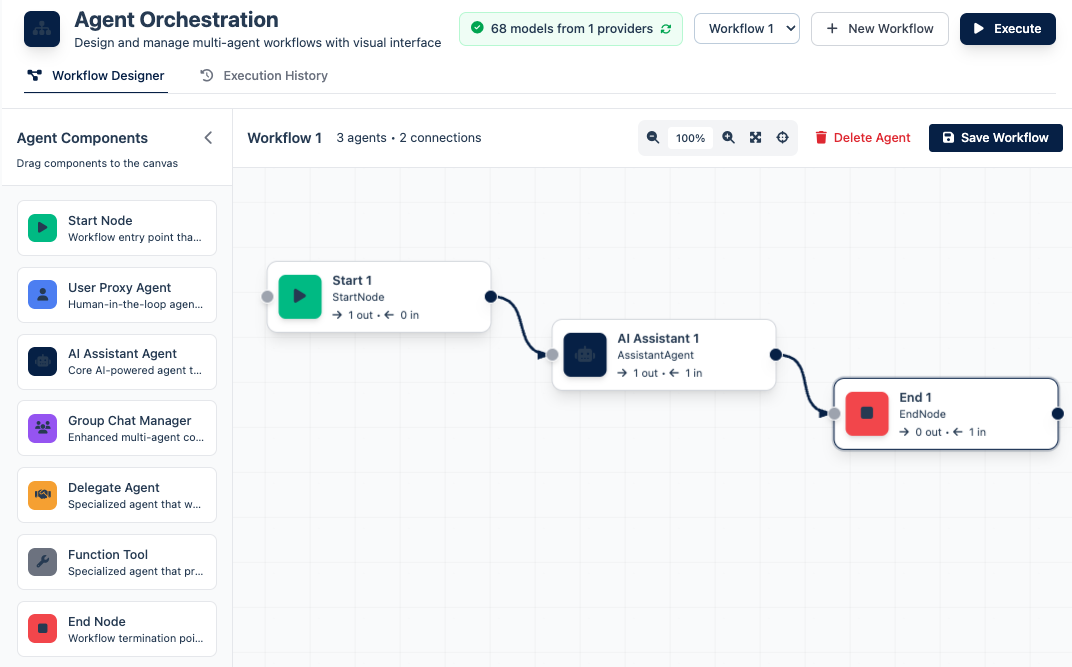
\includegraphics[width=0.9\textwidth]{Figure1_VisualWorkflow.png}
    \caption{Visual Workflow Designer interface showing drag-and-drop canvas with agent nodes and configuration panels. Users connect nodes with edges to define workflow logic and configure per-agent properties including DocAware settings and LLM models.}
    \label{fig:workflow-designer}
\end{figure*}

\subsection{Agent Types}

The framework provides six agent types, each serving distinct roles in workflow orchestration:

\textbf{Start Node} marks the workflow entry point and injects the initial user query into the execution context.

\textbf{AI Assistant Agent} represents an LLM-powered conversational agent with per-agent configurable system prompt, LLM provider selection, model specification, and optional DocAware retrieval. IntelliDoc supports heterogeneous LLM provider deployment within a single workflow: Agent 1 may utilise OpenAI's GPT models \citep{openai2023gpt4}, Agent 2 may employ Anthropic's Claude family \citep{anthropic2024claude}, and Agent 3 may leverage Google's Gemini models \citep{team2023gemini}. This per-agent provider flexibility enables workflows to exploit model-specific capabilities—such as utilising Claude for complex reasoning tasks, GPT-4 for structured output generation, and Gemini for multimodal processing—within a unified orchestration pipeline. Each AI Assistant maintains independent DocAware configurations, allowing simultaneous heterogeneity across both LLM providers and document retrieval strategies.

\textbf{User Proxy Agent} implements human-in-the-loop functionality (Section~\ref{sec:hitl}), pausing workflow execution for human input with two modes: Admin-in-the-Loop for oversight and User-in-the-Loop for end-user interaction.

\textbf{Group Chat Manager} coordinates multiple delegate agents using either round-robin iteration or intelligent delegation with query decomposition (Section~\ref{sec:delegation}). The manager itself operates as an LLM-powered agent with independent provider and model configuration.

\textbf{Delegate Agent} operates as a specialised sub-agent under Group Chat Manager supervision, with its own system prompt, LLM provider and model configuration, and DocAware settings enabling domain-specific retrieval. Each delegate may employ a distinct LLM provider optimised for its specialisation domain.

\textbf{End Node} marks workflow termination, aggregating outputs from connected predecessor nodes and returning the final result.


\section{DocAware: Per-Agent RAG Configuration}
\label{sec:docaware}

DocAware distinguishes IntelliDoc from workflow-level RAG approaches by enabling each agent to independently configure: (1) whether DocAware is enabled, (2) which search method to use, (3) search parameters, and (4) content filters specifying accessible folders and files. Figure~\ref{fig:docaware-config} illustrates the per-agent configuration interface.

\begin{figure}[!t]
    \centering
    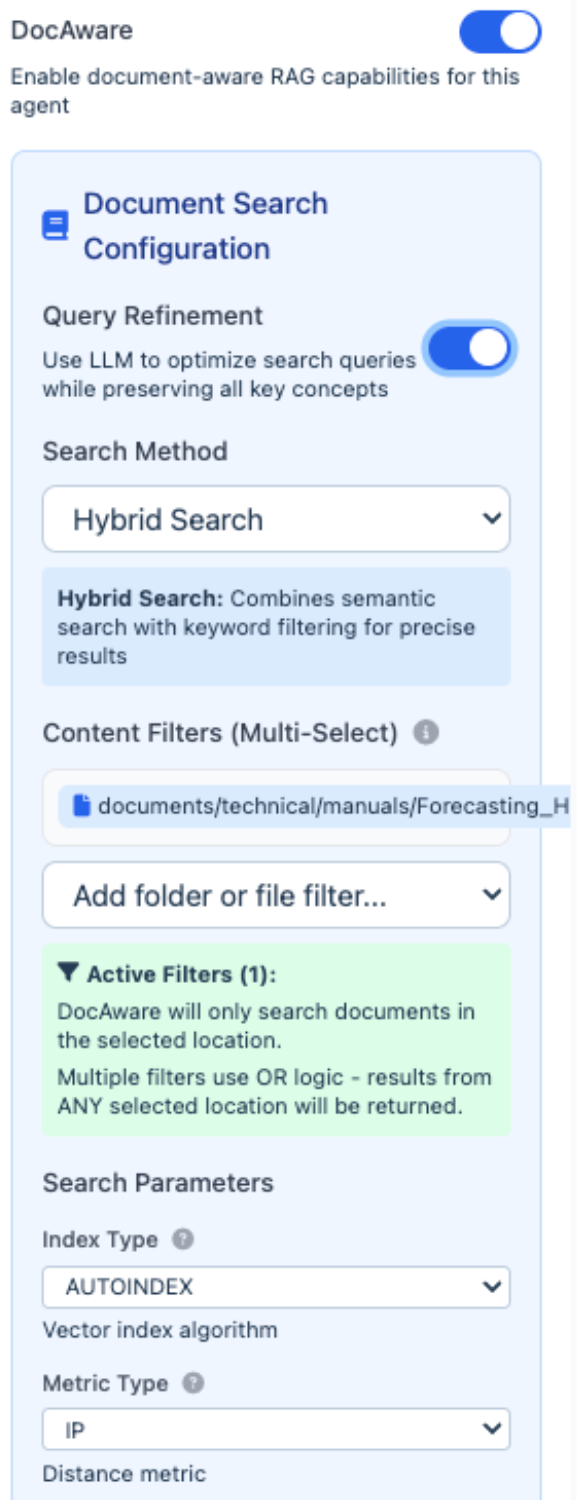
\includegraphics[width=\columnwidth]{Figure2_DocAware.png}
    \caption{Per-agent DocAware configuration interface (Section~\ref{sec:docaware}) enabling independent search method selection and content filtering per agent.}
    \label{fig:docaware-config}
\end{figure}

\subsection{Per-Agent Configuration Model}

Each agent in a workflow can independently configure its DocAware settings, enabling document specialisation impossible with workflow-level RAG systems. For example, a Legal Agent can exclusively access contract folders using hierarchical search, while a Technical Agent searches documentation folders with hybrid retrieval, and a Summary Agent operates without any document retrieval. This per-agent flexibility allows specialised agents to focus on their domain-specific document subsets.

When an agent with DocAware enabled executes, the system extracts a search query from the agent's input context, applies the configured search method with content filters, and injects retrieved documents into the prompt before LLM generation.

\subsection{Content Filtering with Hierarchical Structure}

DocAware extracts hierarchical structure from document filenames during ingestion. A document uploaded as \texttt{Legal/Contracts/Agreement.pdf} creates the virtual path \texttt{Legal/Contracts/} with hierarchical metadata stored in Milvus, enabling prefix-based folder filtering. Content filters support multi-select with OR logic, allowing agents to access multiple folder paths or specific file IDs (see Appendix~\ref{app:content-filter} for filter expression examples).

DocAware integrates with Milvus to support six search strategies including semantic, hybrid, contextual, hierarchical, keyword, and threshold-based search. Each agent selects its optimal strategy based on its specialisation. Details of each search method are provided in Appendix~\ref{app:search-methods}.


\section{Dual-Mode Human-in-the-Loop}
\label{sec:hitl}

The UserProxyAgent implements human-in-the-loop functionality with two distinct modes addressing different deployment contexts. Figure~\ref{fig:hitl-modes} illustrates both Admin-in-the-Loop and User-in-the-Loop interfaces.

\begin{figure}[!t]
    \centering
    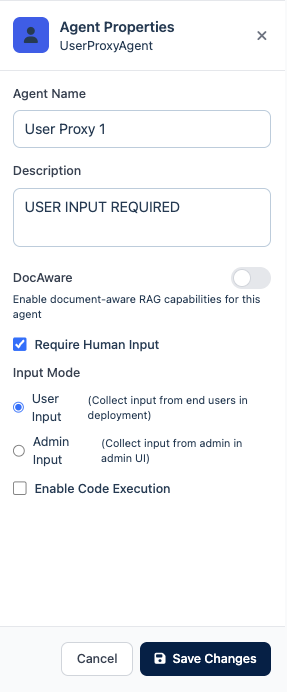
\includegraphics[width=\columnwidth]{Figure3_DualInputMode.png}
    \caption{Dual-mode Human-in-the-Loop interface (Section~\ref{sec:hitl}). Left: Admin-in-the-Loop mode with full workflow context. Right: User-in-the-Loop conversational interface.}
    \label{fig:hitl-modes}
\end{figure}

\subsection{Admin-in-the-Loop Mode}

Admin-in-the-Loop pauses workflow execution for administrator review before responses reach end-users. The administrator interface displays aggregated inputs from connected agents, agent reasoning and intermediate outputs, retrieved documents from DocAware, and the proposed response. This mode enables compliance-critical workflows where human experts must approve AI-generated content before delivery.

\subsection{User-in-the-Loop Mode}

User-in-the-Loop enables stateful conversations in deployed chatbots where end-users provide input mid-workflow. When execution reaches a UserProxyAgent in this mode, the system pauses and creates a \texttt{HumanInputInteraction} record storing execution context. The chatbot presents an input interface, receives user input through the deployment API, and resumes execution with user input as the node's output.


\section{Intelligent Delegation}
\label{sec:delegation}

The Group Chat Manager coordinates multiple delegate agents using two strategies: \textit{round-robin} (iterative cycling) and \textit{intelligent} (LLM-based query decomposition with capability matching). Intelligent delegation is the novel contribution enabling dynamic task distribution (see Figure~\ref{fig:delegation} in Appendix~\ref{app:figures}).

\subsection{Delegation Strategies}

\textbf{Round-Robin Delegation} cycles through all connected delegates for a configurable number of iterations, with each delegate processing the full input context. This suits collaborative refinement where specialists contribute sequentially.

\textbf{Intelligent Delegation} analyzes input queries, decomposes them into subqueries, and routes each to the most capable delegate(s). A query about ``contract terms and technical specifications'' can be split and routed to Legal and Technical delegates respectively.

\subsection{Query Analysis, Matching, and Execution}

The intelligent delegation pipeline consists of three phases. First, \textit{Query Analysis}: given input text and delegate descriptions, the Query Analysis Service uses an LLM to generate structured subqueries, each containing the decomposed query text, priority level, dependencies on other subqueries, and suggested delegates. Second, \textit{Delegate Matching}: for each subquery, the system matches against delegate descriptions using semantic similarity (Algorithm~\ref{alg:match-delegates} in Appendix~\ref{app:delegation-algorithms}). If confidence falls below a threshold (default 0.7), the system broadcasts to all delegates rather than risk incorrect routing. Third, \textit{Parallel Execution}: subqueries are grouped by dependency level using topological sorting (Algorithm~\ref{alg:group-dependencies} in Appendix~\ref{app:delegation-algorithms}); independent subqueries execute in parallel while dependent ones wait for prerequisites.

Algorithm~\ref{alg:intelligent-delegation} details the complete process.

\begin{algorithm}[t]
\caption{Intelligent Delegation}
\label{alg:intelligent-delegation}
\begin{algorithmic}[1]
\REQUIRE Query $q$, delegates $D$, confidence threshold $\theta$
\ENSURE Aggregated delegate responses
\STATE \textit{// Phase 1: Query Analysis}
\STATE $S \leftarrow$ LLM\_SplitQuery($q$)
\STATE \COMMENT{$S$ = list of (id, text, priority, dependencies)}
\STATE
\STATE \textit{// Phase 2: Delegate Matching (see Alg.~\ref{alg:match-delegates})}
\FOR{each subquery $s \in S$}
    \STATE $(delegates, conf) \leftarrow$ MatchToDelegates($s$.text, $D$)
    \IF{$conf < \theta$}
        \STATE $assigned[s] \leftarrow D$ \COMMENT{Broadcast fallback}
    \ELSE
        \STATE $assigned[s] \leftarrow delegates$
    \ENDIF
\ENDFOR
\STATE
\STATE \textit{// Phase 3: Dependency-Aware Execution (see Alg.~\ref{alg:group-dependencies})}
\STATE $levels \leftarrow$ GroupByDependencyLevel($S$)
\FOR{each $level$ in $levels$}
    \STATE $results[level] \leftarrow$ ParallelExecute($assigned$, $level$)
\ENDFOR
\RETURN Aggregate($results$)
\end{algorithmic}
\end{algorithm}


\section{Workflow Evaluation Platform}
\label{sec:evaluation}

IntelliDoc includes an integrated evaluation platform enabling users to assess workflow quality against ground-truth datasets, supporting iterative workflow improvement (see Figure~\ref{fig:evaluation} in Appendix~\ref{app:figures}).

\subsection{Evaluation Methodology}

Users upload CSV files with \texttt{input} and \texttt{expected\_output} columns. For each row, the system: (1) substitutes the Start node prompt with the input, (2) executes the complete workflow, (3) extracts output from nodes connected to the End node, and (4) compares against expected output using multiple metrics.

\subsection{Evaluation Metrics}

The platform computes six metrics: \textbf{ROUGE-1, ROUGE-2, ROUGE-L} for n-gram overlap; \textbf{BLEU} for precision-based evaluation; \textbf{BERTScore} for contextual embedding similarity; and \textbf{Semantic Similarity} using sentence-transformer cosine similarity. Results are stored in database records enabling historical comparison across workflow iterations.


\section{Workflow-to-Chatbot Deployment}
\label{sec:deployment}

IntelliDoc provides a complete deployment pipeline from visual workflow design to embeddable chatbot (see Figure~\ref{fig:deployment} in Appendix~\ref{app:figures}).

\subsection{Deployment Pipeline}

The six-stage pipeline consists of: (1) \textit{Visual Design}—users create workflows via drag-and-drop; (2) \textit{Validation}—graphs are validated for DAG properties and required nodes; (3) \textit{Configuration}—users select the workflow, specify allowed origins, and set rate limits; (4) \textit{Code Generation}—the system generates self-contained HTML embed code; (5) \textit{Integration}—users copy embed code into websites; (6) \textit{Execution}—the system validates origins, enforces rate limits, and executes workflows.

\subsection{Origin Management and Rate Limiting}

Each deployment maintains allowed origins (domains) that can embed the chatbot. The system validates \texttt{Origin} headers, rejecting requests from unlisted domains. Each origin has independent rate limit configuration enabling fine-grained usage control. CORS middleware handles cross-origin requests for browser security compliance. See Appendix~\ref{app:deployment-config} for configuration examples and Appendix~\ref{app:embed-code} for the HTML embed code structure.


\section{Limitations and Conclusion}
\label{sec:conclusion}

\textbf{Limitations.} The intelligent delegation strategy depends on LLM quality for query splitting—poor decomposition may route subqueries incorrectly. Evaluation metrics assess textual similarity but may not capture semantic correctness for all use cases. Documents sent to external LLM providers are subject to those providers' data handling policies.

\textbf{Conclusion.} We presented IntelliDoc, a framework addressing fragmentation between multi-agent orchestration, document retrieval, and chatbot deployment. The five contributions—per-agent DocAware configuration, dual-mode human-in-the-loop, intelligent delegation with query decomposition, workflow evaluation, and seamless deployment—create an end-to-end solution for document-intelligent conversational applications. The per-agent RAG configuration enables specialisation that workflow-level approaches cannot achieve. Intelligent delegation dynamically decomposes complex queries and routes them to capable delegates, advancing beyond static assignment strategies. IntelliDoc will be released as open source.


\section*{Acknowledgements}

We thank the open-source community for foundational tools including Django, SvelteKit, Milvus, and the Hugging Face ecosystem.


% Bibliography must appear before appendix
\bibliographystyle{acl_natbib}
\bibliography{custom}

% Appendix section - appears after references
\clearpage
\appendix

\section{Implementation Details}
\label{app:implementation}

IntelliDoc is implemented with the following technology stack:

\textbf{Backend}: Django 5.2 with Django REST Framework, Celery for background tasks, and asyncio for concurrent workflow execution.

\textbf{Vector Database}: Milvus 2.6.0 with project-specific collections using the pattern \texttt{\{project\_name\}\_\{project\_id\}}. Document embeddings use all-MiniLM-L6-v2 (384 dimensions).

\textbf{Frontend}: SvelteKit with a visual workflow designer supporting drag-and-drop node placement and per-node configuration panels.

\textbf{LLM Integration}: Abstracted provider interface supporting OpenAI, Anthropic, and Google through project-specific API key management with encrypted storage.


\section{Intelligent Delegation Algorithms}
\label{app:delegation-algorithms}

This section provides detailed algorithms for the MatchToDelegates and GroupByDependencyLevel procedures referenced in Algorithm~\ref{alg:intelligent-delegation}.

\subsection{Delegate Matching Algorithm}

Algorithm~\ref{alg:match-delegates} details the semantic similarity-based matching process for routing subqueries to capable delegates.

\begin{algorithm}[h]
\caption{MatchToDelegates: Semantic Capability Matching}
\label{alg:match-delegates}
\begin{algorithmic}[1]
\REQUIRE Subquery text $s$, delegate set $D$, embedding function $\phi$
\ENSURE (matched\_delegates, confidence\_score)
\STATE $q_{emb} \leftarrow \phi(s)$ \COMMENT{Embed subquery}
\STATE $scores \leftarrow []$
\FOR{each delegate $d \in D$}
    \STATE $d_{emb} \leftarrow \phi(d.\text{description})$ \COMMENT{Embed delegate description}
    \STATE $sim \leftarrow \frac{q_{emb} \cdot d_{emb}}{\|q_{emb}\| \|d_{emb}\|}$ \COMMENT{Cosine similarity}
    \STATE Append $(d, sim)$ to $scores$
\ENDFOR
\STATE Sort $scores$ by similarity (descending)
\STATE $top\_delegates \leftarrow$ Select delegates with $sim \geq 0.5$ \COMMENT{Minimum threshold}
\STATE $confidence \leftarrow \max(scores)$ \COMMENT{Highest similarity score}
\RETURN ($top\_delegates$, $confidence$)
\end{algorithmic}
\end{algorithm}

The algorithm computes cosine similarity between the subquery embedding and each delegate's description embedding. Delegates exceeding a minimum similarity threshold (0.5) are selected, with the confidence score being the maximum similarity. If no delegate exceeds the threshold, the confidence will be low, triggering the broadcast fallback in Algorithm~\ref{alg:intelligent-delegation}.

\subsection{Dependency-Based Grouping Algorithm}

Algorithm~\ref{alg:group-dependencies} performs topological sorting to group subqueries by dependency level, enabling parallel execution of independent subqueries.

\begin{algorithm}[h]
\caption{GroupByDependencyLevel: Topological Sort for Parallel Execution}
\label{alg:group-dependencies}
\begin{algorithmic}[1]
\REQUIRE Subquery set $S$ with dependencies
\ENSURE List of dependency levels $L$ where $L[i]$ contains independent subqueries
\STATE $in\_degree \leftarrow \{\}$ \COMMENT{Count incoming dependencies}
\STATE $adj\_list \leftarrow \{\}$ \COMMENT{Adjacency list of dependencies}
\FOR{each subquery $s \in S$}
    \STATE $in\_degree[s] \leftarrow |s.\text{dependencies}|$
    \FOR{each dependency $d \in s.\text{dependencies}$}
        \STATE Add $s$ to $adj\_list[d]$
    \ENDFOR
\ENDFOR
\STATE
\STATE $levels \leftarrow []$
\STATE $current\_level \leftarrow \{s \in S : in\_degree[s] = 0\}$ \COMMENT{No dependencies}
\WHILE{$current\_level \neq \emptyset$}
    \STATE Append $current\_level$ to $levels$
    \STATE $next\_level \leftarrow \emptyset$
    \FOR{each $s \in current\_level$}
        \FOR{each $successor \in adj\_list[s]$}
            \STATE $in\_degree[successor] \leftarrow in\_degree[successor] - 1$
            \IF{$in\_degree[successor] = 0$}
                \STATE Add $successor$ to $next\_level$
            \ENDIF
        \ENDFOR
    \ENDFOR
    \STATE $current\_level \leftarrow next\_level$
\ENDWHILE
\RETURN $levels$
\end{algorithmic}
\end{algorithm}

The algorithm uses Kahn's algorithm for topological sorting. Subqueries with no dependencies form the first level and execute immediately. As each level completes, dependent subqueries have their in-degree decremented; when in-degree reaches zero, they become ready for execution in the next level. This ensures dependent subqueries receive outputs from their prerequisites before executing.


\section{DocAware Search Methods}
\label{app:search-methods}

DocAware integrates with Milvus to support six search strategies:

\begin{enumerate}
    \item \textbf{Semantic Search}: Cosine similarity on document embeddings
    \item \textbf{Hybrid Search}: Combines semantic and keyword matching with configurable weights
    \item \textbf{Contextual Search}: Query expansion using conversation history
    \item \textbf{Hierarchical Search}: Leverages filename-based folder structure for boosting
    \item \textbf{Keyword Search}: BM25-style lexical ranking
    \item \textbf{Threshold Search}: Filters results by minimum similarity score
\end{enumerate}

All methods support hierarchical content filtering, enabling targeted retrieval from specific folder structures.


\section{Content Filter Expressions}
\label{app:content-filter}

Content filters support folder and file-level filtering with OR logic:

\begin{lstlisting}[language=Python,caption={Content filter expression examples}]
# Single folder filter
filter = 'hierarchical_path like "Legal/Contracts%"'

# Multiple folders with OR logic
filter = (
  'hierarchical_path like "Legal/Contracts%"'
  ' or hierarchical_path like "Legal/Policies%"'
)

# Combined folder and file filter
filter = (
  'hierarchical_path like "Reports%"'
  ' or document_id == "doc_12345"'
)
\end{lstlisting}


\section{Deployment Configuration}
\label{app:deployment-config}

Table~\ref{tab:deployment-origins} shows an example per-origin deployment configuration.

\begin{table}[h]
\centering
\small
\begin{tabular}{lcc}
\toprule
\textbf{Allowed Origin} & \textbf{Rate Limit} & \textbf{Status} \\
\midrule
\texttt{example.com} & 60/min & Active \\
\texttt{app.example.com} & 120/min & Active \\
\texttt{staging.example.com} & 30/min & Inactive \\
\bottomrule
\end{tabular}
\caption{Per-origin deployment configuration showing independent rate limits and activation status.}
\label{tab:deployment-origins}
\end{table}


\section{HTML Embed Code Structure}
\label{app:embed-code}

The generated embed code is self-contained:

\begin{lstlisting}[language=HTML,caption={Generated HTML embed code structure}]
<div id="aicc-chatbot">
  <script>
    window.AICC_CONFIG = {
      endpoint: '/api/deploy/{id}/chat/',
      sessionId: crypto.randomUUID(),
      greeting: 'Hello! How can I help?'
    };
  </script>
  <script src="/static/chatbot.js"></script>
</div>
\end{lstlisting}

The chatbot interface includes responsive design, message styling, input handling, error states, and session management for stateful conversations.


\section{System Interface Screenshots}
\label{app:figures}

This section provides detailed interface screenshots for key system components referenced throughout the paper. Figures are displayed in full-width format to show the complete user interface and workflow details. Each screenshot demonstrates specific features discussed in the corresponding main text sections.

\begin{figure*}[t]
    \centering
    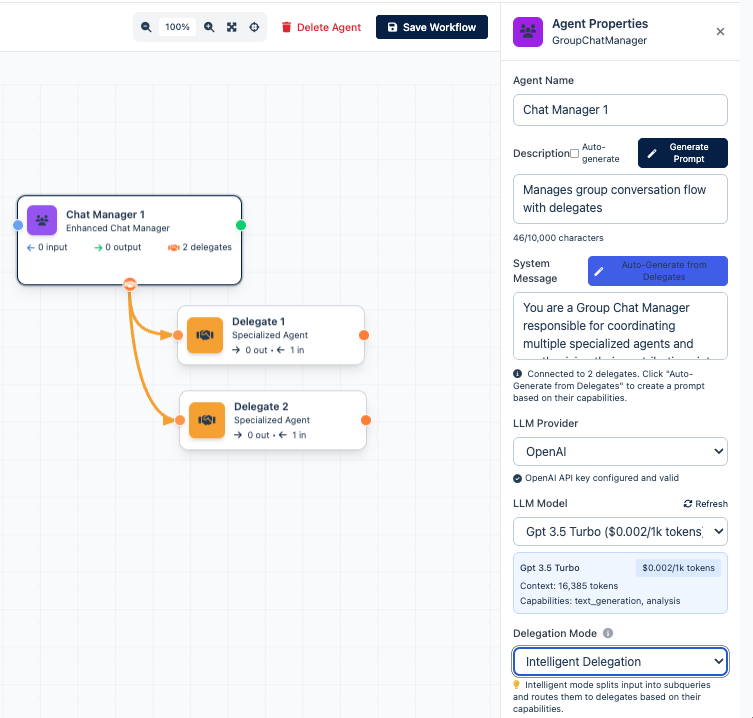
\includegraphics[width=0.9\textwidth]{Figure4_Intelligent_Delegation_Mode.png}
    \caption{Intelligent Delegation workflow visualisation (Section~\ref{sec:delegation}). The interface demonstrates the complete intelligent delegation pipeline: (1) query decomposition into independent and dependent subqueries, (2) semantic capability matching using cosine similarity between subquery embeddings and delegate descriptions, (3) dependency analysis for execution ordering via topological sorting, and (4) parallel execution of independent subqueries while respecting dependencies. The Group Chat Manager aggregates results from all specialised delegates to produce comprehensive responses.}
    \label{fig:delegation}
\end{figure*}

\begin{figure*}[!htbp]
    \centering
    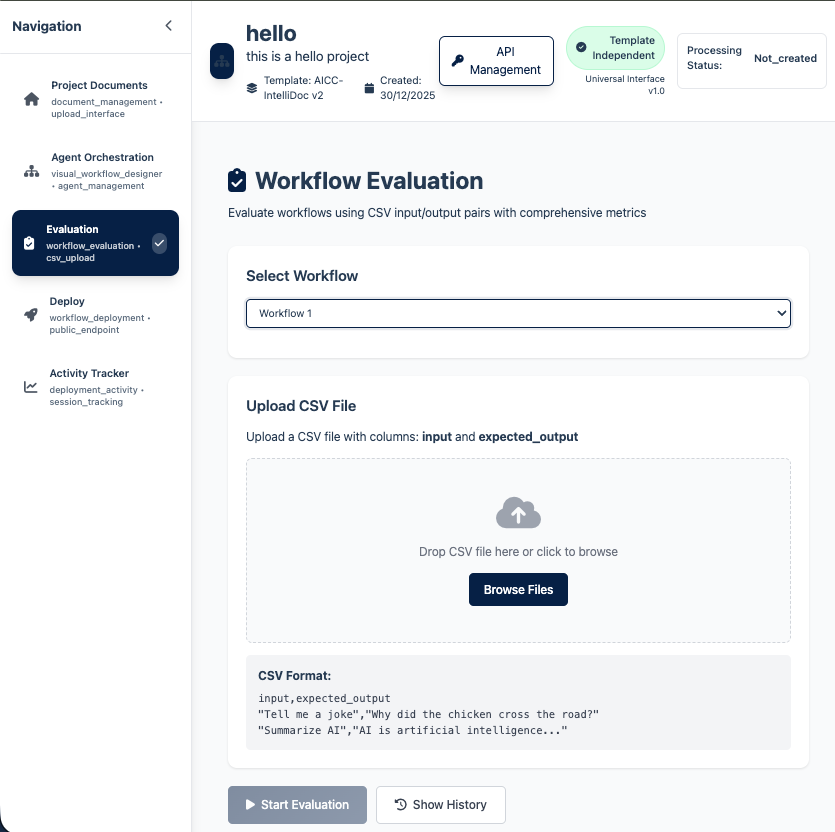
\includegraphics[width=0.9\textwidth]{Figure5_Workflow_Evaluation.png}
    \caption{Workflow Evaluation Platform interface (Section~\ref{sec:evaluation}). The platform enables iterative workflow refinement through comprehensive quality assessment. Users upload CSV datasets containing input-output test pairs, execute workflows against each test case, and receive multi-dimensional quality scores: ROUGE-1/2/L for n-gram overlap assessment, BLEU for precision-based evaluation, BERTScore for contextual embedding similarity, and semantic similarity using sentence transformers. Historical comparison across workflow versions enables data-driven optimisation of agent configurations and prompts.}
    \label{fig:evaluation}
\end{figure*}

\begin{figure*}[!htbp]
    \centering
    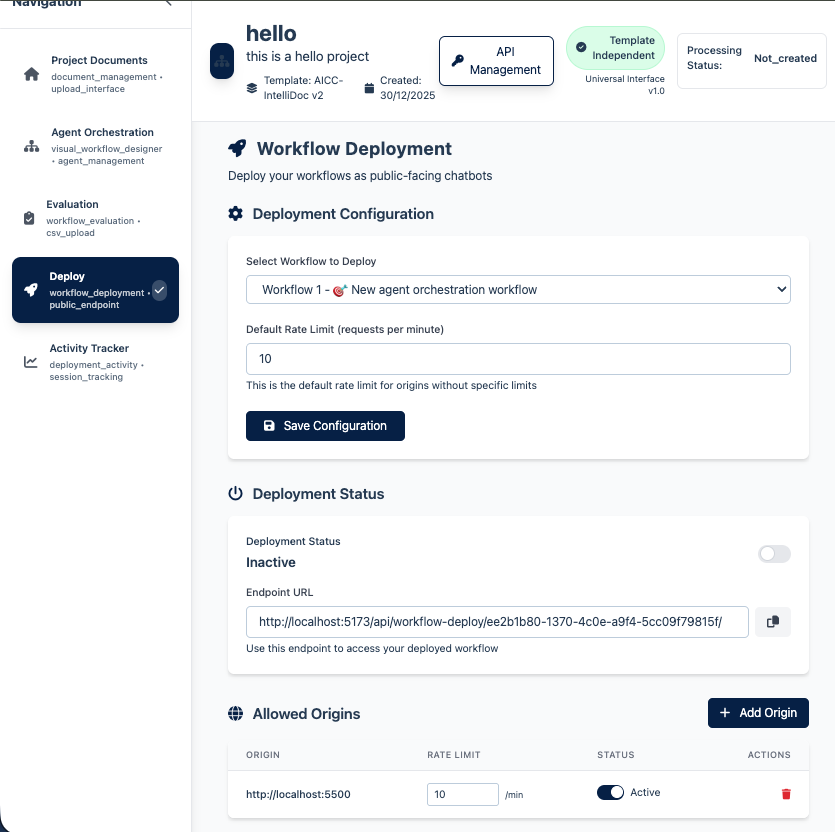
\includegraphics[width=0.9\textwidth]{Figure6_Deployment_Configuration.png}
    \caption{Deployment configuration interface (Section~\ref{sec:deployment}). The deployment system transforms visual workflows into production-ready embeddable chatbots. Administrators specify allowed origins (domains) authorized to embed the chatbot, configure independent rate limits per origin for fine-grained usage control, and receive auto-generated self-contained HTML embed code. The CORS middleware validates origin headers at runtime, enforcing both origin restrictions and rate limits. The deployment supports stateful conversations with session management and handles human-in-the-loop interactions for User Proxy agents.}
    \label{fig:deployment}
\end{figure*}


\end{document}
